\documentclass{minimal}
\usepackage{tikz}
\usetikzlibrary{shapes}

\begin{document}

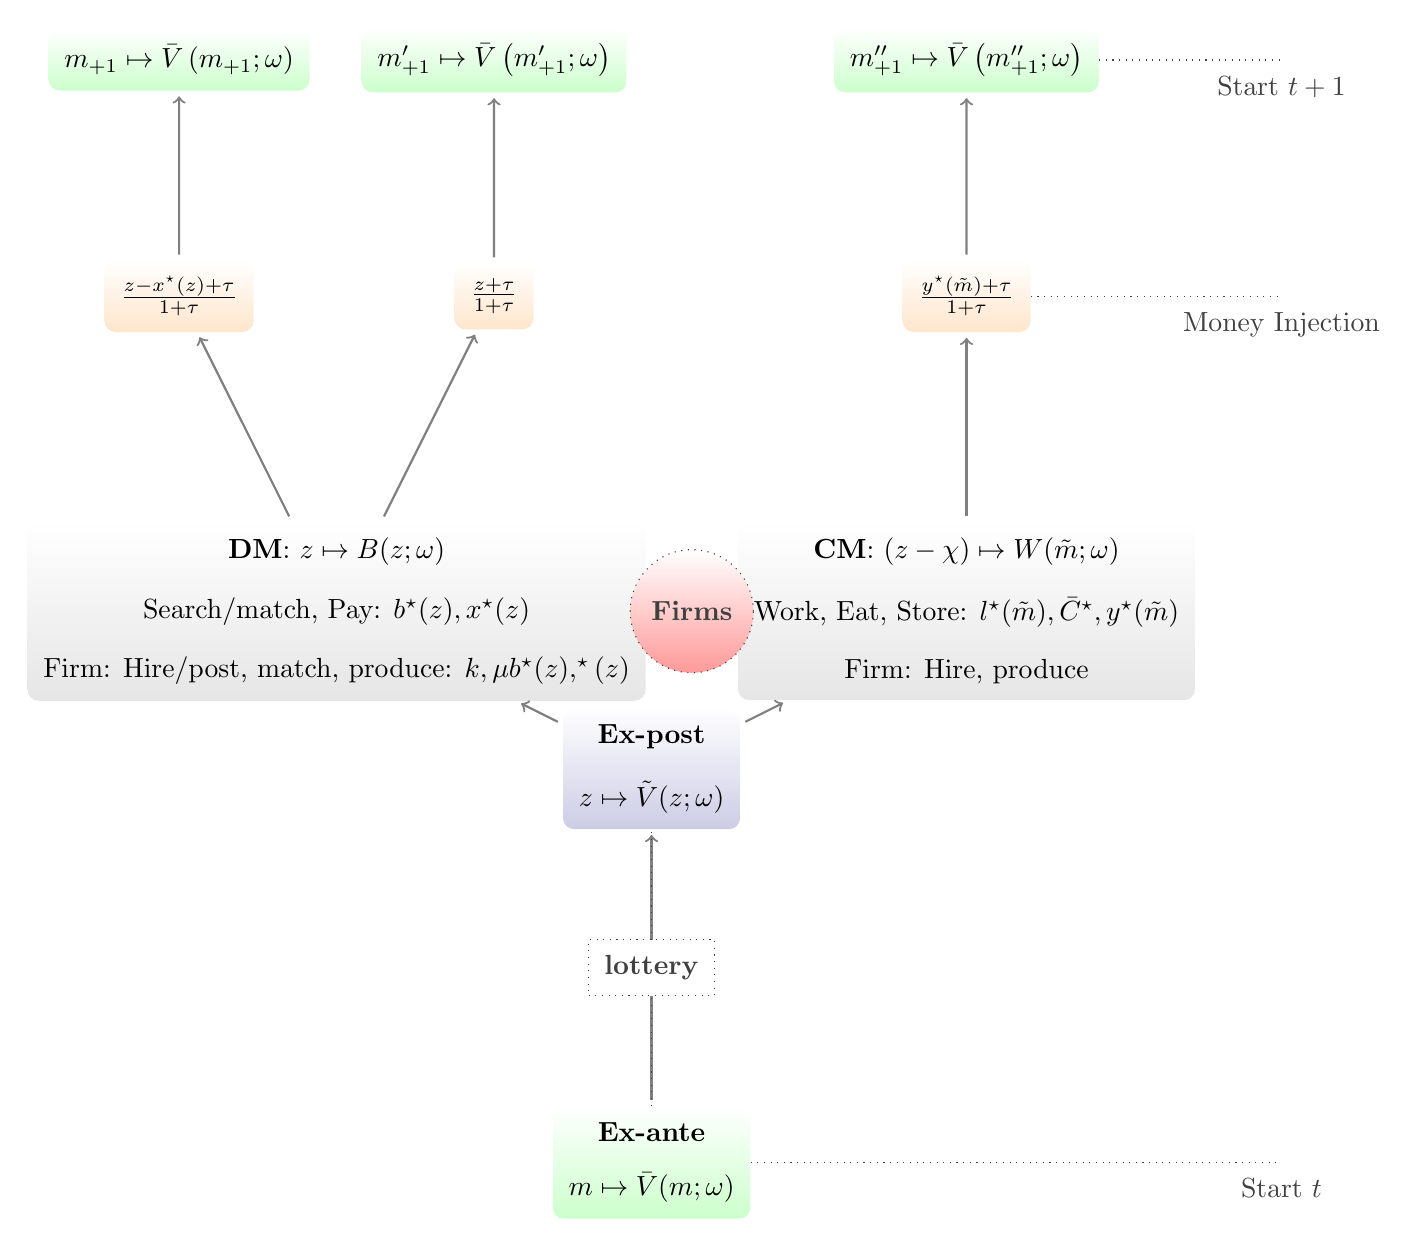
\begin{tikzpicture}[
        rotate=90,
        % Individual Child Level Settings
        level 1/.style={  sibling distance=6cm,level distance=5cm,
                          bottom color=green!80!blue!20!white, top color=white
                        },
        level 2/.style={  sibling distance=8cm, level distance=2.0cm,
                          top color=white,
                          bottom color=blue!50!black!20,
                          draw=blue!40!black!60,
                          very thick
                        },
        level 3/.style={sibling distance=4cm, level distance=4.0cm},
        level 4/.style={  sibling distance=2cm, level distance=3.0cm,
                          bottom color=green!80!blue!20!white,
                          top color=white
                        },
        % Edge between Nodes style
        edge from parent/.style={thick,draw=gray,shorten >=2pt, shorten <=2pt,->},
        % COlorscheme for Nodes
        kant/.style={text width=1cm, text centered, sloped},
        every node/.style={text ragged, inner sep=2mm},
        daft/.style={ rectangle, rounded corners, shade, top color=white,
                      bottom color=green!20!white, draw=none, very thin
                    },
        punkt/.style={  rectangle, rounded corners, shade, top color=white,
                        bottom color=blue!50!black!20, draw=none, very thin
                        },
        kraft/.style={  rectangle, rounded corners, shade, top color=white,
                        bottom color=gray!20!white, draw=none, very thin
                        },
        werk/.style={  rectangle, rounded corners, shade, top color=white,
                        bottom color=orange!20!white, draw=none, very thin
                        },
        louboutin/.style={  rectangle, rounded corners, shade, top color=white,
                        bottom color=red!20!white, draw=none, very thin
                        }
]
  % Parent
  \node[daft, rectangle split, rectangle split parts=2]
        (home) {  \textbf{Ex-ante}
                  \nodepart{second}
                  $m \mapsto \bar{V}(m; \omega)$
                }
  [grow=right]
    % Child 1
    child {
      node[punkt, rectangle split, rectangle split parts=2]
          (lottery) {  \textbf{Ex-post}
                    \nodepart{second}
                    $z \mapsto \tilde{V}(z; \omega)$
                  }
      % START: Child Level 2 - DOWN (CM activities)
      child {node [kraft, rectangle split, rectangle split parts=3]
            (CM) {  \textbf{CM}: $(z - \chi) \mapsto W(\tilde{m};\omega)$
                      \nodepart{second}
                      Work, Eat, Store: $l^{\star}(\tilde{m}), \bar{C}^{\star}, y^{\star}(\tilde{m})$
                      \nodepart{third}
                      Firm: Hire, produce
                    }
        % Child 3-DOWN <- 2-DOWN
        child[grow=0] {
          node[werk] (CMresid) {$\frac{y^{\star}(\tilde{m})+\tau}{1+\tau}$
          }
          % Agent from CM
          child {
            node[daft] (CMout) {
                          $m_{+1}^{\prime\prime} \mapsto \bar{V}\left(
                          m_{+1}^{\prime\prime}; \omega
                          \right)$
                        }
          } % END: Child Level 4 - DOWN
        } % END: Child Level 3 - DOWN
      } % END: Child Level 2 - DOWN
      % START: Child Level 2 - UP (DM activities)
      child {node[kraft] [rectangle split, rectangle split parts=3]
            (DM) {  \textbf{DM}: $z \mapsto B(z;\omega)$
                      \nodepart{second}
                      Search/match, Pay: $b^{\star}(z), x^{\star}(z)$
                      \nodepart{third}
                      Firm: Hire/post, match, produce: $k, \mu b^{\star}(z), \circq^{\star}(z)$
                    }
        % Child 3-DOWN <- 2-UP (Agent not matched)
        child {
          node[werk] {$\frac{z + \tau}{1+\tau}$}
          % Child 4-DOWN <- 3-DOWN <- 2-UP
          child {
            node[daft] (DMoutA) {
                            $m_{+1}^{\prime} \mapsto
                            \bar{V}\left(
                            m_{+1}^{\prime}; \omega
                            \right)$
                          }
          }
        }
        % Child 3-UP <- 2-UP (Agent matched)
        child {node[werk] {$\frac{z-x^{\star}(z)+\tau}{1+\tau}$}
          % Child 4-DOWN <- 3-UP <- 2-UP
          child {node[daft] (DMoutB) {
                                      $m_{+1} \mapsto \bar{V}\left(
                                      m_{+1}; \omega
                                      \right)$
                                      }
          }
        }
      %edge from parent[double]
    } % END: Child level 1
  }; % End PARENT
  % Label below Parent (Home)
  \draw[dotted,gray!50!black] ([yshift=-4cm]home) -- +(0,-4) node[below]{Start $t$};
  % Label below btw Parent (home) and Ex-Post (lottery)
  \draw[dotted,gray!50!black] (home) -- (lottery)
    node[midway, rectangle, draw, midway, fill=white] {\textbf{lottery}};
      %child[grow=90] {node[left] {Possible lottery}};
  % Label for Firm
  \draw[dotted,gray!50!black, <->] (DM) -- (CM)
    node[midway, circle, draw, bottom color=red!40!white, top color=white] {\textbf{Firms}};
      %child[grow=0] {node[left] {Firm: CM and DM}};
  % Label below Final first sibling of Level 4 child
  \draw[dotted,gray!50!black] ([yshift=-4cm]CMresid) -- +(0,0) node[below]{Money Injection};

  % Label below Final first sibling of Level 4 child
  \draw[dotted,gray!50!black] ([yshift=-4cm]CMout) -- +(0,0)
  node[below]{Start $t+1$};
\end{tikzpicture}

\end{document}
